\documentclass[a4paper, top=10mm]{article}
%for writing from the top
\usepackage{fullpage}
%for math
\usepackage{amsmath}
\usepackage{mathrsfs}
\usepackage{amsthm}
%for images
\usepackage{graphicx}
%for color
\usepackage{xcolor}
%for title
\title{\textbf{\huge{Cinema}}}
\author{Enigma n\textsuperscript{o}1}
\date{2\textsuperscript{nd} December 2022}

\newtheorem*{hint}{Hint}

\addtolength{\voffset}{-2cm}
\addtolength{\textheight}{5cm}


\begin{document}
	\maketitle
	
	We start with testing your mathematical cinema knowledge.
	
	"It's My Turn" is a 1980 American romantic comedy-drama film starring Jill Clayburgh, Michael Douglas, and Charles Grodin.
	The film was directed by Claudia Weill and written by Eleanor Bergstein.
	
	Kate Gunzinger is a mathematics professor at a Chicago university. She lives with divorcé Homer, in a comfortable but not terribly passionate relationship.
	Kate travels to New York for a job interview and to attend the wedding of her widowed father. She is offered the job, though it does not look promising, as she will not be able to continue doing research. She meets the bride's son, Ben Lewin, a former professional baseball player.
	Ben is married, but a relationship develops with Kate. He takes her to Yankee Stadium for an old-timers' day ceremony, and eventually, they have an affair. When they part, Kate goes back to Chicago and breaks up with Homer. She returns to work, where she is greeted with a gift sent by Ben.
	
	\begin{center}
		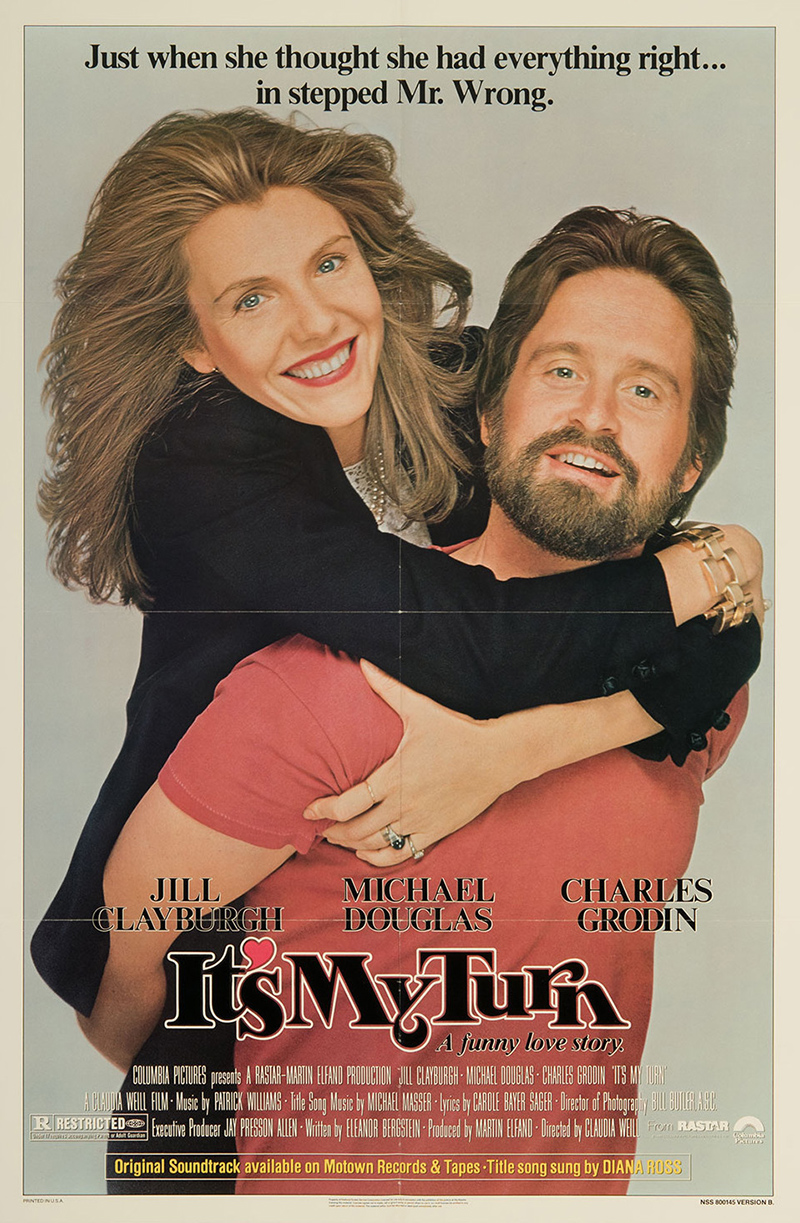
\includegraphics[height=270pt]{01its_my_turn.jpg}\\
		"It's my turn" movie poster.
	\end{center}


	In the movie, one famous mathematical statement is proved (and the proof showed in the movie is actually valid!).
	
	\textbf{What is the name of this statement?}
	\footnote{The answer box is non-case-nor-white-space-sensitive.}
	
	\begin{hint}
		The statement is named after an animal.
	\end{hint}


	
\end{document}